\documentclass[twoside,11pt]{article}

% jmlr2e.sty already loads epsfig, amssymb, natbib (plainnat), graphicx and
% hyperref, and defines proof/theorem environments. Load additional packages
% after it.
\usepackage{jmlr2e}

\usepackage{amsmath}
\usepackage{booktabs}
\usepackage{multirow}
\usepackage{lastpage}
\usepackage[expansion=false]{microtype}

% Allow slightly looser lines so long hyphenated compounds do not overflow.
\setlength{\emergencystretch}{2em}

% Handy macros
\newcommand{\x}{\mathbf{x}}
\newcommand{\xh}{\hat{\mathbf{x}}}
\newcommand{\z}{\mathbf{z}}
\newcommand{\R}{\mathbb{R}}
\newcommand{\Lrec}{\mathcal{L}_{\mathrm{rec}}}
\newcommand{\LKL}{\mathcal{L}_{\mathrm{KL}}}
\newcommand{\LSAM}{\mathcal{L}_{\mathrm{SAM}}}
\newcommand{\lphys}{\lambda_{\mathrm{phys}}}
\newcommand{\Qn}{Q2$^{n}$}

% Heading arguments are
%   {volume}{year}{pages}{date submitted}{date published}{paper id}{author-full-names}
% Volume, dates and paper id are assigned by JMLR; placeholders until then.
% TODO(authors): replace "Author One and Author Two" with the full author list.
\jmlrheading{--}{2026}{1-\pageref{LastPage}}{--}{--}{--}{Author One and Author Two}

% Short headings: running title (odd pages) and authors' last names (even pages)
% TODO(authors): replace "One and Two" with the authors' last names.
\ShortHeadings{Disentangling the Spectrum with PRISM}{One and Two}
\firstpageno{1}

\begin{document}

\title{Disentangling the Spectrum with PRISM: A Dual-Stream Physics-Informed VAE for Decoupled Representational Learning of Hyperspectral Images}

% TODO(authors): replace placeholders with real names, affiliations and emails.
\author{\name Author One \email one@example.com \\
       \addr Department\\
       Institution\\
       City, Country
       \AND
       \name Author Two \email two@example.com \\
       \addr Department\\
       Institution\\
       City, Country}

\editor{TBD}

\maketitle

% TODO: JMLR caps the abstract at 200 words; this one (ported verbatim) is ~216.
\begin{abstract}%   <- trailing '%' for backward compatibility of .sty file
Hyperspectral imaging (HSI) captures dense reflectance spectra across hundreds of contiguous spectral bands. Robust representation learning of this data is central to applications like remote sensing, mineral mapping, atmospheric characterization etc. However sensor degradation, transmission failures, and external noise routinely corrupt these cubes, motivating a need for variational representation learning, typically via VAEs, to compress and probabilistically reconstruct corrupted spectra. Conventional VAEs apply convolutions that mix spatial and spectral information indiscriminately, blurring spectral signatures and causing posterior collapse or physically improbable hallucinations. Thus, we introduce PRISM (Physics-Informed Representation for Isolated Spectral-Spatial Modeling). PRISM is a dual-stream VAE routing spatial and spectral information through two independently-supervised spatial and spectral branches that re-couple only under a Spectral Angle Mapper (SAM) bounded fusion. This lets PRISM retain the spatial fidelity of standard 2D VAEs without sacrificing chemical accuracy; gaining up to $4.72$~dB PSNR over the strongest rival architecture on each dataset while matching the best spectral angle in the grid to within $0.05^\circ$, and leading every dataset on the combined spatial-spectral quality index \Qn. This decoupled latent is designed as a backbone for Latent Diffusion Models (LDMs) for purifying deep-space transmission corruptions and generating omitted frames. It already supports chemical interpolation for mineral discovery while offering a scalable framework for other physics-heavy domains like precision agriculture and climatology.
\end{abstract}

% TODO: JMLR requires exactly five keywords.
\begin{keywords}
  keyword one, keyword two, keyword three, keyword four, keyword five
\end{keywords}

% =========================================================================
\section{Introduction}
\label{sec:intro}

Hyperspectral images (HSI) are imaging spectrometer products which record a continuous reflectance spectrum sampled across hundreds of thin contiguous wavelength bands per pixel. An HSI sensor resolves the fine spectral structure like absorption dips, peaks and continuum slopes that is a representation of the diagnostics of physical and chemical composition of surface imaged. A single HSI cube therefore provides a spatial image and per pixel spectroscopic measurement simultaneously.

This dual nature of hyperspectral images makes them important across a wide range of remote-sensing domains. For terrestrial remote sensing, HSI underlines precision agriculture like crop stress and nutrient mapping \citep{wang2024npk}, environmental and atmospheric monitoring \citep{stuart2019environmental}, and mineral exploration \citep{bedini2017mineral}. Astronomical imaging spectrometers such as the Chandrayaan-2 Imaging Infra-Red Spectrometer (IIRS) \citep{chowdhury2020iirs} and the Compact Reconnaissance Imaging Spectrometer for Mars (CRISM) \citep{murchie2007crism} are the primary instruments used to map lunar and Martian surface mineralogy and hydration state from orbit, while airborne sensors such as AVIRIS \citep{green1998aviris} are used to map vegetation, soil, and mineral composition and monitor coastal water quality, extending the same hyperspectral toolkit from planetary orbit down to Earth's surface.

An HSI cube is large in size and expensive to transmit and store in full, representation learning has become a key aspect of working with it by compressing the HSI cube into a compact latent representation to learn embeddings for downstream tasks. Recently, representation learning has evolved towards producing latent inputs required by modeling frameworks such as Latent Diffusion Models (LDMs) \citep{rombach2022ldm} as their starting point rather than operating on full-resolution pixels directly. Autoencoders \citep{hinton2006reducing} are a proven architecture for image compression for a long time. However, simple compression is not enough for real HSI data. Sensor degradation, transmission dropouts, and instrument or environmental noise routinely corrupt cubes, so a useful latent must not only encode a clean cube but also plausibly \emph{repair or regenerate} its corrupted or missing parts. This is where we move towards Variational Autoencoders (VAEs) \citep{kingma2014vae} as a natural candidate. VAEs learn a smooth, regularized latent space instead of discrete fragments, such that they can interpolate between observations and probabilistically regenerate spectra they have not seen verbatim. This makes them well suited to denoising corrupted patches \citep{im2017denoising}, filling missing regions \citep{peng2021inpainting}, and synthesizing chemically plausible signatures between known materials \citep{gomezbombarelli2018chemical}.

The standard convolutional VAE underperforms on these capabilities when processing HSI cubes because it treats them as an RGB image. 2D convolutions over the spatial $(H, W)$ plane, applied to hundreds of bands, mix spatial neighborhoods and spectral channels indiscriminately. The inductive bias in CNNs suits spatial structure but not spectral fidelity. It blurs the absorption features that carry chemical meaning, and under the tight bottleneck that a VAE requires, it leads to posterior collapse \citep{bowman2016generating} or to reconstructions that are spatially plausible but chemically wrong. The result is a conflict between spatial and spectral fidelity that a single-stream convolutional VAE cannot resolve. For downstream scientific analysis that depends on these learned bottlenecks, such hallucinations are a grave artifact.

For resolving this conflict, we introduce PRISM (Physics-Informed Representation for Isolated Spectral-Spatial Modeling). PRISM is a dual-stream VAE that routes spatial and spectral information via two independently-supervised encoder-decoder branches, and combines their reconstructions at a physics-bounded fusion step constrained by a differentiable Spectral Angle Mapper (SAM) penalty. This ensures that a spatial denoiser and a spectral-fidelity model are each free to specialize, and are only ever combined under a term that directly penalizes the chemical hallucinations which a naive fusion would otherwise permit.

Our main contributions are:
\begin{enumerate}
  \item A split-stream architecture for self-supervised representation learning of hyperspectral cubes, where spatial and spectral reconstructions are re-coupled at a single physics constraint fusion step, which penalizes chemically-hallucinated reconstructions directly rather than relying on reconstruction error alone.
  \item A falsification-oriented ablation protocol leveraging latent-rate matching, posterior-collapse detection, a spatial-reliance shuffle test and a downstream-readiness benchmark suite that includes latent noise-injection robustness, chemical-interpolation smoothness, and spectral band-masking recovery; which evaluate PRISM's bottlenecks as a potential LDM backbone.
\end{enumerate}

% =========================================================================
\section{Related Works}
\label{sec:related}

\paragraph{Representation learning and spectral unmixing for HSI:}
A large body of work applies representation learning to hyperspectral data for compression and spectral unmixing. Convolutional architectures adapted from standard image based models learn joint spatial-spectral information directly from raw cubes \citep{chen2016deep}, and hybrid spatial-spectral CNNs such as HybridSN \citep{roy2020hybridsn} combine 3D and 2D convolutions in a single feature hierarchy to trade off the two kinds of structure. Recently, Transformer-based encoders have been proposed to model long-range spectral dependencies directly, as in SpectralFormer \citep{hong2022spectralformer}, while spatial-spectral recurrent transformers have been used specifically for HSI denoising and restoration \citep{fu2024sst}, alongside convolutional restoration networks such as HSI-DeNet \citep{chang2019hsidenet}. Autoencoder-based unmixing recovers a small set of endmember spectra and per-pixel abundances via an objective that is close to representation learning even though it does not model a generative latent space \citep{su2019daen,palsson2018unmixing}. The Spectral Angle Mapper (SAM) itself, which PRISM adopts as a fusion-bounding loss, originates in this classical spectral-matching literature \citep{kruse1993sips} stating that it measures spectral distortion regardless of what architecture is used to produce a reconstruction.

\paragraph{Differentiable physics-penalty training:}
A separate line of work constrains network outputs with a differentiable physical prior rather than relying on architecture or capacity alone to enforce physical plausibility. Physics-informed neural networks or PINNs \citep{raissi2019pinn} add a residual of governing directly into the objective function so that the network's output is penalized whenever it violates known physics. In remote sensing, physics-guided autoencoders for planetary spectroscopy have used a radiative-transfer model as a differentiable penalty during unmixing of lunar hyperspectral data \citep{lin2026hapke}, which motivates the idea for PRISM's SAM-bounded fusion.

\paragraph{Split-stream and decoupled architectures within HSI:}
% NOTE(typo-review): "split without." is left as in the source draft; intended wording unclear.
Several HSI-specific architectures have worked with explicit spatial-spectral split without. FactoFormer \citep{mohamed2023factoformer} factorizes a hyperspectral transformer into separately pretrained spectral and spatial transformer branches, each with its own masked self-supervised objective that fuses their learned representations only for downstream classification. S2ADet \citep{he2023s2adet} also decouples spectral and spatial information at the input via a dedicated decoupling module before routing it through a two-stream feature-extraction network for hyperspectral object detection, arguing that treating the two axes jointly from the start discards their complementary structure. \citet{du2024modality} shows that decoupling shared and complementary information between a low-resolution hyperspectral image and a high-resolution multispectral image rather than fusing them directly is sufficient for strong unsupervised fusion performance using a substantially lighter network than prior fusion architectures. These works provide the basis for the structural intuition PRISM builds on for representation learning, i.e.\ spatial and spectral information degrade each other when processed jointly, and separating them into dedicated branches recovers signal that a joint architecture loses.

\paragraph{Split-stream architectures beyond hyperspectral imagery:}
Split stream architectures are used far beyond the domain of remote sensing and hyperspectral imagery. \citet{simonyan2014twostream} introduced this concept for video action recognition, training separate spatial (appearance) and temporal (motion) streams, and combining their predictions by late fusion. Within VAE specifically, \citet{lee2021privateshared} disentangle private latent spaces specific to modality from a shared latent space across multiple data modalities using a PoE (Product of Experts) inference network. \citet{guo2024dualvae} apply an analogous dual-branch disentangled VAE to separately model user and item side latent factors for collaborative recommendation. \citep{boukun2025multistream} proposes a multi-stream VAE that gives each data source its own independently-supervised stream, recombined through a learned combination model, applied to separating superimposed digits and mixed acoustic sources. The setting differs in terms of separate sources in a mixture, not separate axes of one input, but the underlying design choice is the same one PRISM makes for HSI; let each stream specialize, then recombine them late under an explicit, learned criterion for how much to trust each.

% =========================================================================
\section{Methodology}
\label{sec:method}

% TODO(JMLR): JMLR style forbids a heading directly following another heading;
% add a short lead-in sentence here before \subsection{PRISM Architecture}.

\subsection{PRISM Architecture}
\label{sec:arch}

Given an input patch $\x \in \R^{64\times64\times C}$ (where $C$ is the sensor's band count), a \emph{spatial stream} and a \emph{spectral stream} each independently encode, reparameterize, and decode a reconstruction of the patch. The reconstructions are combined only at the final, physics-bounded fusion step as shown in Figure~\ref{fig:pipeline} and Figure~\ref{fig:network}.

\paragraph{Spatial stream}
is responsible for preserving and denoising spatial context. The encoder begins with a $3{\times}3$ convolution that projects the input $C$-band spectrum onto a 64-channel local representation while mixing the spectrum of a pixel with its neighbors. Three strided ($s=2$) convolutional blocks then progressively halve the resolution of the $64{\times}64$ patch down to $8{\times}8$ while widening the channel dimension, and a final pointwise convolution outputs the mean and log-variance of the latent. The decoder mirrors this path and upsamples the spatial latent ($\z_s$) back to full resolution with transposed convolutions and mapping the features back to $C$ bands through a sigmoid output.

\begin{figure}[t]
  \centering
  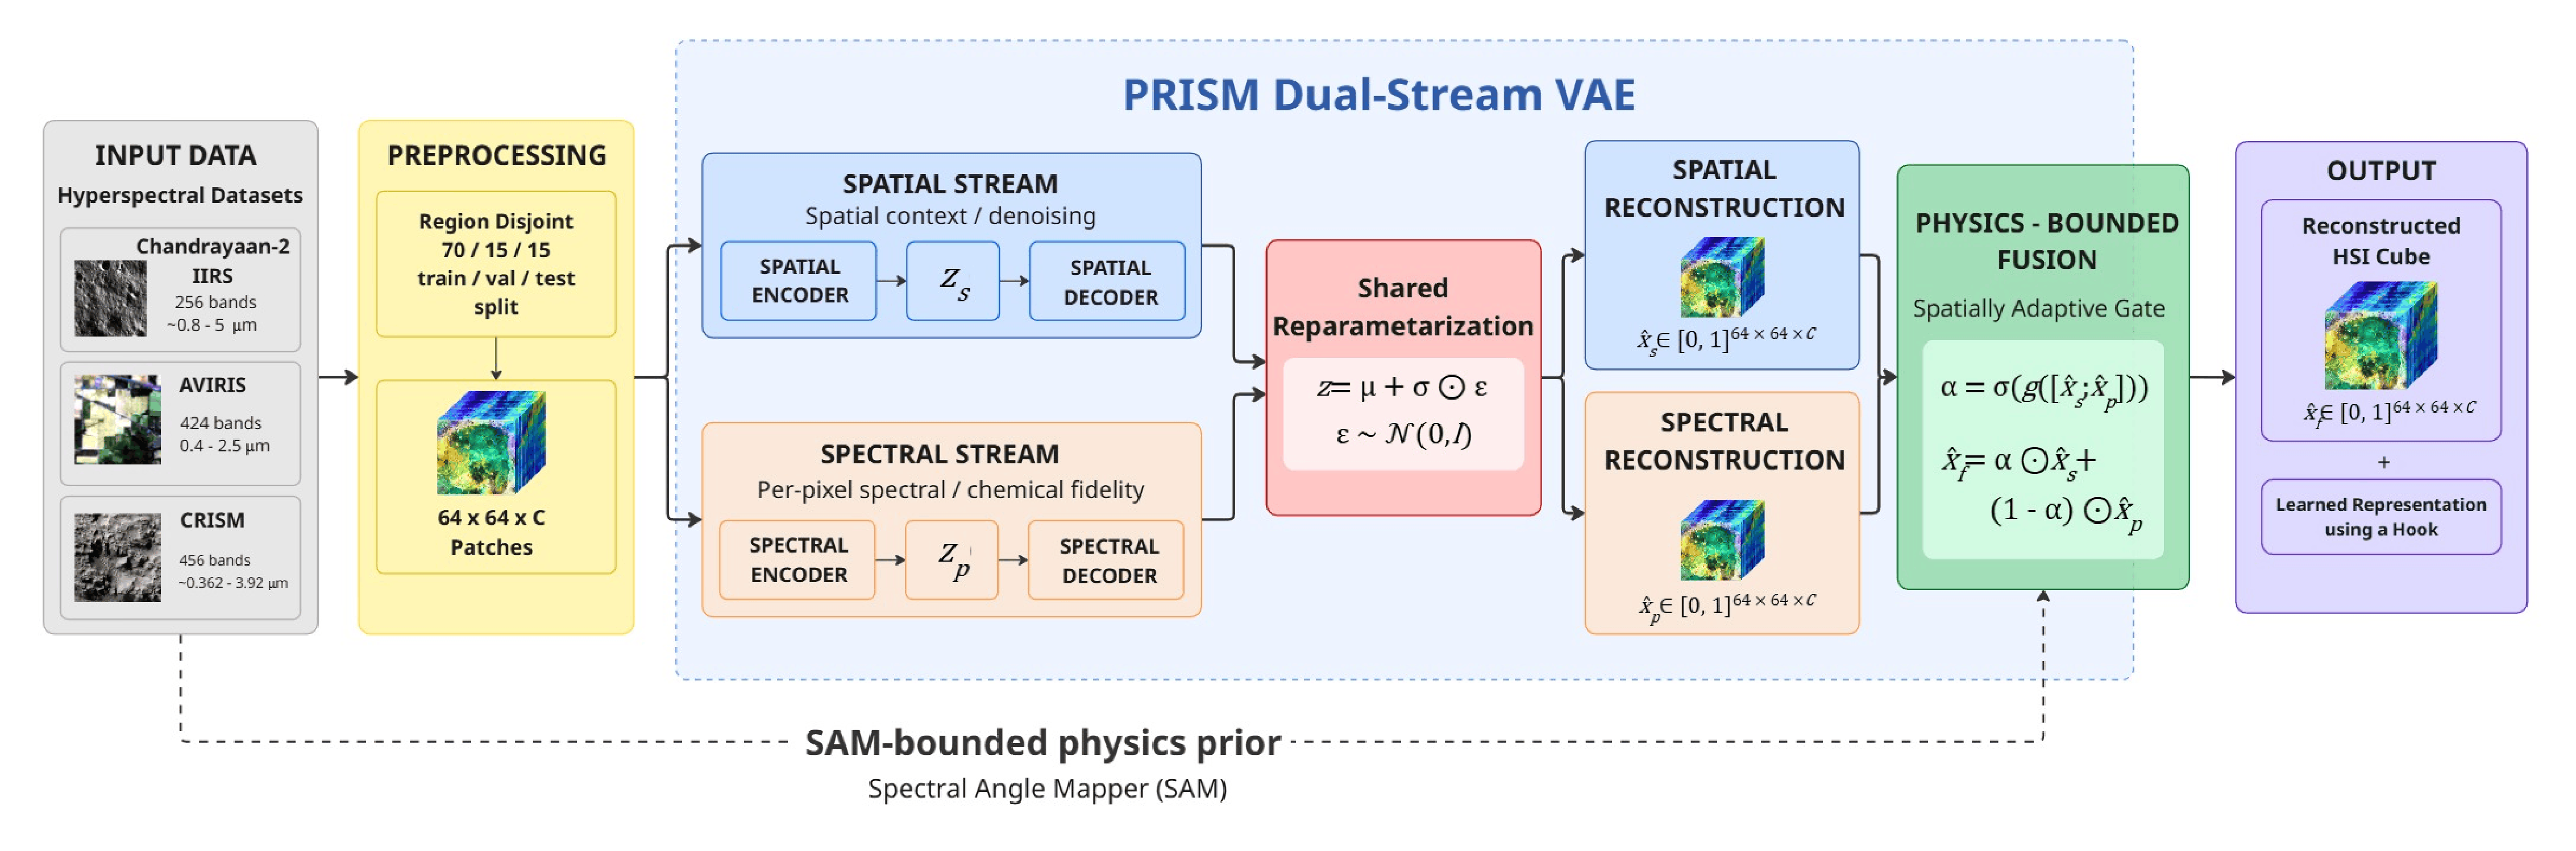
\includegraphics[width=\textwidth]{figures/prism_pipeline.png}
  \caption{Pipeline of PRISM for representation learning of HSI}
  \label{fig:pipeline}
\end{figure}

The latent $\z_s \in \R^{d_s\times8\times8}$, where $d_s$ is a dataset specific spatial latent width, is an addressable spatial map rather than a single global vector, so the spatial stream can vary the texture, shapes and contrast information across the patch.

\paragraph{Spectral stream}
is responsible for per-pixel chemical information processing. It never mixes information across pixels because a pixel's chemical signature is a critical entity. The encoder applies two strided ($s=2$) 1D convolutions along the spectral axis with $\mathrm{ReLU}$ activation which channels ($1\rightarrow32\rightarrow64$) then flattens and projects through a linear layer to a $2d_p$-dimensional mean/log-variance vector per pixel, where $d_p$ is a dataset specific latent width. The per pixel outputs are reshaped back onto the spatial grid, which gives a per-pixel latent map $\z_p \in \R^{d_p\times H\times W}$. The decoder mirrors the encoder with two strided ($s=2$) 1D transposed convolutions, ending in a sigmoid. As every layer in this stream operates on one pixel at a time, the spectral stream architecturally prevents colluding one pixel's spectrum with another.

Both encoders output a $(\mu, \log\sigma)$ pair, chunked along the channel axis. A single shared reparameterization function samples $\z = \boldsymbol{\mu} + \boldsymbol{\sigma}\odot\boldsymbol{\varepsilon}$, such that $\boldsymbol{\varepsilon}\sim\mathcal{N}(0,\,I)$, with $\log\sigma$ clamped to $[-30, 20]$ for numerical stability. The said function is applied identically to $\z_s$ and $\z_p$. Each stream produces its own full reconstruction of the patch, $\xh_s$ and $\xh_p$, both bounded in $[0,1]$. We need to combine them because they encode separate information, the spatial stream is better at encoding edges and texture, while the spectral stream is stronger at preserving per pixel spectral shape. Instead of averaging them with a fixed weight, PRISM lets a small two-layer $3{\times}3$ convolutional network $g$ look at both reconstructions side by side and decide, for every pixel and every band, how much to trust each one. Passing $g(\cdot)$ through a sigmoid gives $\boldsymbol{\alpha} = \sigma(g([\xh_s;\xh_p]))$ such that values near 1 favor the spatial stream and values near 0 favor the spectral stream. The fused reconstruction is then a weighted blend of the two:
\begin{equation}
  \xh_f = \boldsymbol{\alpha}\odot\xh_s + (1-\boldsymbol{\alpha})\odot\xh_p.
  \label{eq:fusion}
\end{equation}
However this carries a risk. By taking some bands mostly from one stream and others mostly from the other, $\alpha(\cdot)$ could splice together a spectrum whose shape matches neither $x_s$ nor $x_p$, thus lowering reconstruction error while pointing in the wrong direction chemically. The gate is therefore trained jointly with the rest of the network under the SAM term, which penalizes exactly this kind of angular distortion.

\begin{figure}[t]
  \centering
  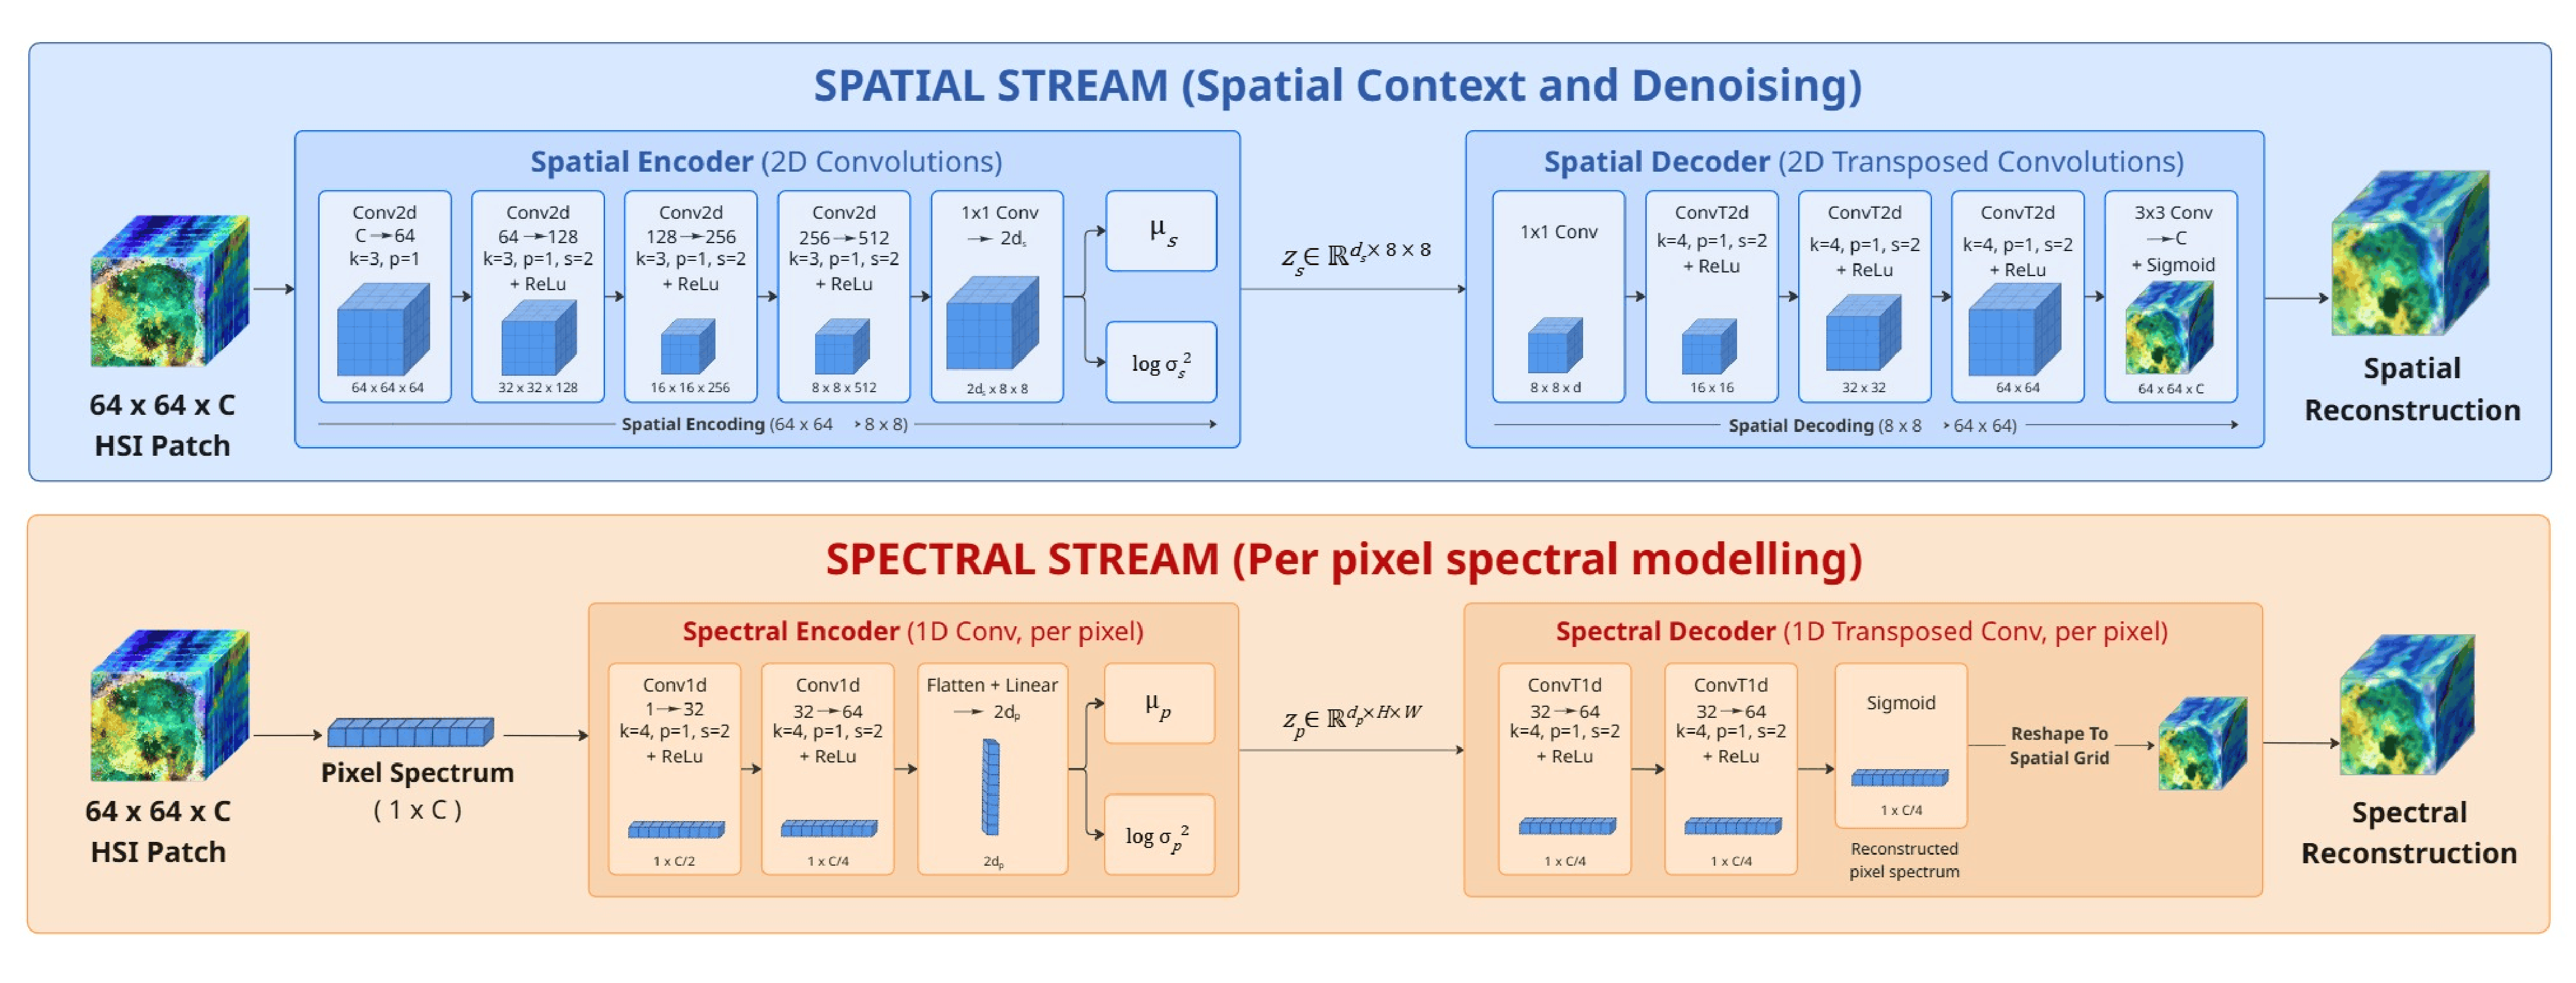
\includegraphics[width=\textwidth]{figures/prism_network.png}
  \caption{Network structure of PRISM}
  \label{fig:network}
\end{figure}

\subsection{Objective Function and Physics-Informed Fusion}
\label{sec:objective}

PRISM's training objective is a standard multi-term evidence lower bound (ELBO) \citep{jordan1999variational} with an added SAM penalty term. The closed form of the objective is
\begin{equation}
  \mathcal{L} = \Lrec + \beta\,\LKL + \lphys\,\LSAM,
  \label{eq:objective}
\end{equation}
with $\beta=10^{-3}$ and $\lphys=0.3$ held constant throughout training (no annealing) and identical across every model and dataset in the ablation grid.

$\Lrec$ is defined as:
\begin{equation}
  \Lrec = \frac{0.5\cdot\mathrm{MSE}(\xh_f,\x) + w\cdot\mathrm{MSE}(\xh_s,\x) + w\cdot\mathrm{MSE}(\xh_p,\x)}{0.5+2w},
  \qquad w = 0.1,
  \label{eq:rec}
\end{equation}
where $\xh_f, \xh_s, \xh_p$ represent the fused, spatial-only, and spectral-only reconstructions respectively. A normalized weighted mean with an effective 5:1:1 ratio between the fused term and each branch's own auxiliary reconstruction term is used. The auxiliary terms ensure that each stream is individually supervised and neither branch can rely entirely on the other to reconstruct the patch. The normalization keeps $\Lrec$ in a scale directly comparable to a single-stream VAE's reconstruction term.

$\LKL$ is likewise a mean over both streams' divergences,
\begin{equation}
  \LKL = \frac{\mathrm{KL}(\z_s) + \mathrm{KL}(\z_p)}{2},
  \qquad
  \mathrm{KL}(\z) = -\frac{1}{2}\,\mathbb{E}\!\left[1 + \log\sigma^2 - \mu^2 - \sigma^2\right],
  \label{eq:kl}
\end{equation}
reduced over every element of the latent so that latent size does not bias the magnitude across streams of different shapes.

$\LSAM$ is the Spectral Angle Mapper, applied only to the \emph{fused} reconstruction. It is defined as:
\begin{equation}
  \LSAM(\x, \xh_f) = \mathbb{E}_{i,j}\,\arccos\!\left(
    \frac{\langle \x_{ij},\, \xh_{f,\,ij}\rangle}
         {\left(\|\x_{ij}\| + \epsilon\right)\left(\|\xh_{f,\,ij}\| + \epsilon\right) + \epsilon}
  \right),
  \quad \epsilon = 10^{-8},
  \label{eq:sam}
\end{equation}
The cosine is additionally clamped to $[-(1-\epsilon),\,1-\epsilon]$ before the arccosine. SAM is invariant to illumination scaling, so it penalizes a reconstruction whose spectral \emph{direction} differs from the input's regardless of its magnitude which is exactly the chemical-hallucination failure mode a naive fusion would otherwise be free to produce.

\noindent\textbf{NOTE:} a pixel whose true spectral energy falls below $\epsilon$ contributes exactly $\pi/2$ to $\LSAM$ irrespective of the model's prediction. We report both the raw SAM and an energy-masked \emph{SAM-valid} that excludes these pixels, and we use SAM-valid for every cross-model and cross-dataset comparison in \S\ref{sec:results}.

\subsection{Experiment Setup}
\label{sec:setup}

\paragraph{Ablation grid:}
PRISM's performance is evaluated against three baseline VAEs, each representing a different way of handling the spectral axis, on terrestrial and astronomical hyperspectral datasets under an identical training pipeline:
\begin{itemize}
  \item \textbf{2D Spatial VAE} adapts Stable Diffusion's \texttt{AutoencoderKL} \citep{rombach2022ldm} to HSI. It treats the cube as a thick image, using only 2D convolutions with no explicit spectral structure, at its original base width of 128 channels over three downsampling stages (23.4--24.5M parameters).
  \item \textbf{3D Spatio-Spectral VAE} follows the fully-3D convolutional autoencoder line for HSI \citep{chen2016deep}. The patch is treated as a single-channel volume, so every kernel spans the spatial and spectral axes at once. We use a base width of 24 filters, representative of this line since the original per-layer filter counts are not recoverable (3.10M parameters).
  \item \textbf{1D Pixelwise VAE} follows the per-pixel spectral autoencoder line \citep{palsson2018unmixing,liu2022dualfreq}. Each pixel's spectrum is encoded independently by a shared four-layer fully-connected network with hidden widths $(512, 256, 128)$, so the model never sees the spatial grid (0.60--0.80M parameters).
\end{itemize}

\begin{table}[t]
  \centering
  \begin{tabular}{llccccc}
    \toprule
    Dataset & Instrument & Bands & Wavelength & Train & Valid & Test \\
    \midrule
    IIRS   & Chandrayaan-2 IIRS & 256 & $\sim$0.8--5.0~$\mu$m & 14,624 & 3,084 & 3,084 \\
    AVIRIS & Airborne AVIRIS    & 424 & 0.4--2.5~$\mu$m       & 11,027 & 2,180 & 1,950 \\
    CRISM  & MRO CRISM          & 456 & 0.362--3.92~$\mu$m    & 2,561  & 369   & 369   \\
    \bottomrule
  \end{tabular}
  \caption{Datasets used in the ablation grid, after preprocessing and patch extraction. 7000 randomly sampled training patches are used for training; for CRISM, we use all the 2,561 patches. Band counts are the number of contiguous reflective channels retained by the packing pipeline (after removing non-reflective or degenerate detector channels), not the raw sensor channel count.}
  \label{tab:datasets}
\end{table}

Baselines keep the widths reported in their respective papers rather than being parameter-matched to PRISM (5.20--5.95M parameters). We match the latent rate for each dataset. Every model's bottleneck is sized to the same total number of latent elements ensuring close to a 64:1 compression ratio (16,384 elements on IIRS at 64.0:1; 28,672 on AVIRIS and CRISM at 60.6:1 and 65.1:1 respectively; the 3D Spatio-Spectral VAE's volumetric bottleneck quantises to 27,136 and 29,184 elements on AVIRIS and CRISM, both at 64.0:1 and well inside the audit tolerance of \S\ref{sec:results}). Hence, no architecture is compared at a looser or tighter bottleneck than another. For seed invariance, every model is trained at two random seeds under the objective of \S\ref{sec:objective}. Moreover, each of the baseline models is trained once under a standard ELBO to isolate the effect of the $\LSAM$ term.

\paragraph{Data pipeline:}
We split each hyperspectral cube into smaller $64{\times}64{\times}C$ cubes (patches), extracted at a stride of 48 pixels (25\% overlap) from region-disjoint 70/15/15 train\slash validation\slash test slices of each source scene, so that a training patch and a test patch are never drawn from adjacent, overlapping terrain. We then create a combined packed set of 7,000 patches (or its full size where smaller) per dataset to train on; validation and test splits are never capped. All models are trained for 60 epochs with AdamW, learning rate $10^{-3}$, 5-epoch linear warm-up followed by cosine annealing, gradient-norm clipped at 1.0.

% =========================================================================
\section{Results and Discussion}
\label{sec:results}

% TODO: results section is not final; content below is carried over from the
% latest ICLR draft as-is, including its bracketed [Pending] notes.
% TODO: FLOP analysis to be added.

\paragraph{Mechanism diagnostics.}
Before comparing architectures, we check that every trained cell reflects a real, non-degenerate model rather than an artifact of the training or evaluation pipeline. Five diagnostics are run on every frozen checkpoint: the first four are reported in Table~\ref{tab:diagnostics}, and the fifth, a spectral band-masking recovery test, in Table~\ref{tab:bandmask}.

\emph{Latent-rate audit} confirms every cell lands within the preregistered $\pm25\%$ tolerance of its dataset's common latent budget $T$ (\S\ref{sec:setup}). This ensures that a rate-unmatched cell cannot be attributed a win or loss on architecture alone, since a looser bottleneck trivially helps reconstruction.

\emph{Posterior-collapse detection} confirms that each model actually uses its latent. A collapsed model ignores its latent code, so its decoder emits a near-constant output regardless of what code it is given. We look for this in two ways: the fraction of latent units carrying non-trivial KL divergence (\emph{Active units}), and a latent-swap test that decodes one patch from a different patch's code, which should change the output substantially if the latent is in use (\emph{Swap $\Delta$}). Cells showing collapse are excluded from every comparison rather than silently scored. In this grid, the 2D Spatial VAE under the standard-ELBO objective is the architecture most prone to collapse because it has no physics term to stop its decoder from settling on a near-constant, low-error output when the reconstruction objective alone permits it.

\emph{Spatial-reliance shuffle} permutes the spatial grid of pixels, keeping each pixel's own spectrum intact, and re-scores the shuffled reconstruction against the shuffled input, reporting the resulting relative SAM degradation. A model that makes no genuine use of spatial context is exactly unaffected by the shuffle, which is why the 1D Pixelwise VAE serves as this diagnostic's positive control because it processes the input pixelwise. Its intact and shuffled scores must match to within the tolerance for exact permutation-equivariance, or else the diagnostic itself is at fault. Its SRI is therefore read first, confirming that the diagnostic measures what it claims to be before any other model's shuffle result is read as a finding.

\begin{table}[t]
  \centering
  \small
  \setlength{\tabcolsep}{4pt}
  \resizebox{\textwidth}{!}{%
  \begin{tabular}{llcccccccccc}
    \toprule
     & & \multicolumn{1}{c}{\textbf{Latent}} & & & \multicolumn{1}{c}{\textbf{Spatial}} & & & & & \\
     & & \multicolumn{1}{c}{\textbf{rate}} & \multicolumn{2}{c}{\textbf{Posterior collapse}} & \multicolumn{1}{c}{\textbf{reliance}} & \multicolumn{5}{c}{\textbf{Trivial-predictor floor}} \\
    \cmidrule(lr){3-3}\cmidrule(lr){4-5}\cmidrule(lr){6-6}\cmidrule(lr){7-11}
    \textbf{Model} & \textbf{Obj.} &
    \textbf{\begin{tabular}[b]{@{}c@{}}Rate\\(.\,:1)\end{tabular}} &
    \textbf{\begin{tabular}[b]{@{}c@{}}Active\\units (\%)$\uparrow$\end{tabular}} &
    \textbf{\begin{tabular}[b]{@{}c@{}}Swap\\$\Delta\uparrow$\end{tabular}} &
    \textbf{SRI} &
    \textbf{\begin{tabular}[b]{@{}c@{}}Floor\\PSNR\end{tabular}} &
    \textbf{\begin{tabular}[b]{@{}c@{}}Lift\\(dB)$\uparrow$\end{tabular}} &
    \textbf{\begin{tabular}[b]{@{}c@{}}Lift SAM-v\\(rel.)$\uparrow$\end{tabular}} &
    \textbf{\begin{tabular}[b]{@{}c@{}}vs.\ mean-\\patch (dB)$\uparrow$\end{tabular}} &
    \textbf{\begin{tabular}[b]{@{}c@{}}Head-\\room$\uparrow$\end{tabular}} \\
    \midrule
    \multicolumn{11}{@{}l}{\textbf{IIRS}} \\
    PRISM & Phys. & \textbf{64.0} & \textbf{99.6} & \textbf{1.739} & \textbf{0.093} & \textbf{30.52} & \textbf{9.70} & \textbf{0.603} & \textbf{3.42} & \textbf{0.108} \\
    \midrule
    \multirow{2}{*}{2D Spatial VAE}         & Phys. & 64.0 & 94.6  & 0.853 & 0.142 & 30.52 & 9.43 & 0.435 & 3.15  & 0.105 \\
                                            & ELBO  & 64.0 & 100.0 & 0.001 & 0.001 & 30.52 & 5.13 & 0.016 & -1.15 & 0.057 \\
    \midrule
    \multirow{2}{*}{3D Spatio-Spectral VAE} & Phys. & 64.0 & 96.6  & 0.502 & 0.128 & 30.52 & 8.55 & 0.332 & 2.27  & 0.096 \\
                                            & ELBO  & 64.0 & 99.9  & 0.070 & 0.021 & 30.52 & 5.81 & 0.001 & -0.47 & 0.065 \\
    \midrule
    \multirow{2}{*}{1D Pixelwise VAE}       & Phys. & 64.0 & 71.6  & 1.812 & 0.000 & 30.52 & 2.51 & 0.605 & -3.77 & 0.028 \\
                                            & ELBO  & 64.0 & 81.2  & 0.046 & 0.000 & 30.52 & 3.75 & 0.044 & -2.53 & 0.042 \\
    \midrule
    \multicolumn{11}{@{}l}{\textbf{AVIRIS}} \\
    PRISM & Phys. & \textbf{60.6} & \textbf{100.0} & \textbf{1.568} & \textbf{0.000} & \textbf{15.95} & \textbf{19.82} & \textbf{0.629} & \textbf{5.67} & \textbf{0.191} \\
    \midrule
    \multirow{2}{*}{2D Spatial VAE}         & Phys. & 60.6 & 100.0 & 0.001 & 0.007 & 15.95 & -1.20 & -0.198 & -15.36 & -0.012 \\
                                            & ELBO  & 60.6 & 100.0 & 0.085 & 0.157 & 15.95 & 13.27 & 0.188  & -0.89  & 0.128 \\
    \midrule
    \multirow{2}{*}{3D Spatio-Spectral VAE} & Phys. & 64.0 & 95.7  & 1.012 & 0.463 & 15.95 & 17.48 & 0.553 & 3.33 & 0.168 \\
                                            & ELBO  & 64.0 & 100.0 & 0.615 & 0.311 & 15.95 & 17.00 & 0.416 & 2.84 & 0.163 \\
    \midrule
    \multirow{2}{*}{1D Pixelwise VAE}       & Phys. & 60.6 & 53.4  & 1.623 & 0.000 & 15.95 & 19.00 & 0.635 & 4.84 & 0.183 \\
                                            & ELBO  & 60.6 & 72.2  & 0.756 & 0.000 & 15.95 & 16.28 & 0.377 & 2.12 & 0.156 \\
    \midrule
    \multicolumn{11}{@{}l}{\textbf{CRISM}} \\
    PRISM & Phys. & \textbf{65.1} & \textbf{100.0} & \textbf{0.054} & \textbf{0.001} & \textbf{11.06} & \textbf{23.04} & \textbf{0.408} & \textbf{15.64} & \textbf{0.212} \\
    \midrule
    \multirow{2}{*}{2D Spatial VAE}         & Phys. & 65.1 & 100.0 & 0.011 & 0.011 & 11.06 & 13.38 & -0.422 & 5.98 & 0.123 \\
                                            & ELBO  & 65.1 & 100.0 & 0.075 & 0.007 & 11.06 & 15.67 & -0.364 & 8.27 & 0.144 \\
    \midrule
    \multirow{2}{*}{3D Spatio-Spectral VAE} & Phys. & 64.0 & 99.9  & 0.077 & 0.086 & 11.06 & 17.82 & 0.366 & 10.42 & 0.164 \\
                                            & ELBO  & 64.0 & 99.1  & 0.151 & 0.016 & 11.06 & 17.77 & 0.040 & 10.37 & 0.163 \\
    \midrule
    \multirow{2}{*}{1D Pixelwise VAE}       & Phys. & 65.1 & 91.8  & 0.031 & 0.000 & 11.06 & 18.32 & 0.171  & 10.92 & 0.168 \\
                                            & ELBO  & 65.1 & 86.0  & 0.044 & 0.000 & 11.06 & 19.35 & -0.115 & 11.95 & 0.178 \\
    \bottomrule
  \end{tabular}
  }
  \caption{Mechanism diagnostics. All values are diagnostic only, with no pass/fail threshold.}
  \label{tab:diagnostics}
\end{table}

\emph{Trivial-predictor floor} asks whether a trained model actually beats predictors that involve no learning at all. The best zero-rate floor is the best of the train-set global, fold, and region mean spectra, which carry no per-patch information (\emph{Floor PSNR}). We report the model's lift over it in PSNR (\emph{Lift}) and in relative SAM-valid (\emph{Lift SAM-v}). The per-patch spatial-mean predictor is a substantially stronger learning-free predictor so the baseline and PRISM's margin over it are reported under \emph{vs.\ mean-patch}. Finally, \emph{Headroom} is the fraction of the gap between the zero-rate floor and an input-copy model that the PRISM and baseline's PSNR actually captures.

With every cell confirmed to be a real, non-degenerate model, we turn to the first question the ablation is designed to answer: how faithfully each architecture reconstructs a clean, held-out cube. Table~\ref{tab:recon} reports reconstruction quality on the held-out test split. PRISM records the highest PSNR on every instrument (40.22, 35.78, 34.10~dB), improving on the strongest rival architecture by 0.27, 0.83 and 4.72~dB, and it leads every dataset on both spatial correlation (SCC) and the combined hypercomplex index \Qn, where its margin ranges from 9 to 17\%. On the spectral axis it is first on CRISM ($2.38^\circ$) and second by $0.05^\circ$ on IIRS and $0.02^\circ$ on AVIRIS, differences smaller than the seed spread we observe, so we read SAM-valid as a three-way tie at the top rather than a loss. Two columns genuinely favour a baseline. SSIM prefers the 3D Spatio-Spectral VAE on IIRS and CRISM, which is expected of a model optimising a volumetric objective directly, though it pays for that structural advantage with two to three times PRISM's pixel error. SID prefers the 3D VAE on CRISM; we report but do not rank CRISM SID, because 53.7\% of its values reach the numerical clamp. [Seed half-ranges and paired significance tests pending the consolidated rerun.]

\begin{table}[t]
  \centering
  \small
  \resizebox{\textwidth}{!}{%
  \begin{tabular}{llccccccc}
    \toprule
    \textbf{Dataset} & \textbf{Model} & \textbf{SAM-valid ($^\circ$)}$\downarrow$ & \textbf{PSNR}$\uparrow$ & \textbf{SSIM}$\uparrow$ & \textbf{SID}$\downarrow$ & \textbf{SCC}$\uparrow$ & \textbf{Q2$^{n}$}$\uparrow$ & \textbf{Params (M)} \\
    \midrule
    \multirow{4}{*}{IIRS}
      & 2D Spatial VAE         & 9.60          & 39.95          & 0.947          & 0.1593          & 0.077          & 0.718          & 23.40 \\
      & 1D Pixelwise VAE       & \textbf{6.70} & 33.03          & 0.845          & \textbf{0.0897} & 0.223          & 0.666          & 0.60 \\
      & 3D Spatio-Spectral VAE & 11.34         & 39.07          & \textbf{0.954} & 0.1940          & 0.104          & 0.572          & 3.10 \\
      & \textbf{PRISM}         & 6.75          & \textbf{40.22} & 0.939          & 0.0914          & \textbf{0.224} & \textbf{0.830} & 5.20 \\
    \midrule
    \multirow{4}{*}{AVIRIS}
      & 2D Spatial VAE         & 5.30          & 14.75          & 0.718          & 0.0212          & 0.000          & 0.123          & 24.38 \\
      & 1D Pixelwise VAE       & \textbf{1.62} & 34.95          & 0.849          & \textbf{0.0014} & 0.455          & 0.805          & 0.77 \\
      & 3D Spatio-Spectral VAE & 1.98          & 33.44          & 0.841          & 0.0028          & 0.091          & 0.676          & 3.10 \\
      & \textbf{PRISM}         & 1.64          & \textbf{35.78} & \textbf{0.871} & 0.0014          & \textbf{0.530} & \textbf{0.878} & 5.85 \\
    \midrule
    \multirow{4}{*}{CRISM}
      & 2D Spatial VAE         & 5.71          & 24.44          & 0.831          & 0.3081          & 0.035          & 0.201          & 24.45 \\
      & 1D Pixelwise VAE       & 3.33          & 29.38          & 0.781          & 0.1595          & 0.310          & 0.329          & 0.80 \\
      & 3D Spatio-Spectral VAE & 2.54          & 28.88          & \textbf{0.940} & \textbf{0.0719} & 0.051          & 0.382          & 3.10 \\
      & \textbf{PRISM}         & \textbf{2.38} & \textbf{34.10} & 0.841          & 0.1649          & \textbf{0.398} & \textbf{0.446} & 5.95 \\
    \bottomrule
  \end{tabular}
  }
  \caption{Reconstruction capability of models on held-out test split. Best value per dataset and column in bold. SID (spectral information divergence) and SCC (spatial correlation coefficient) are reported alongside PSNR/SSIM/SAM to give a fuller spatial-and-spectral fidelity picture. Q2$^{n}$ is a combined hypercomplex quality index \citep{garzelli2009q2n}. Metrics are to be compared meaningfully within a dataset and not across datasets.}
  \label{tab:recon}
\end{table}

Reconstruction of noise free latent does not show how the model behaves when the bottleneck is noised, which matters highly for the intended use of PRISM as a starting point for LDMs. We therefore add a varying amount of Gaussian noise directly to each model's encoded latent and measure how much the reconstruction degrades (Table~\ref{tab:noise}). This is the one axis on which PRISM is measurably worse, and the table is constructed so that fact is visible rather than hidden. At $\sigma{=}0.1$ PRISM is the strongest model on CRISM (30.72~dB) and within 0.07~dB of the best on IIRS, but by $\sigma{=}1.0$ it has given up 12.1, 20.6 and 19.3~dB against its own clean-latent reconstruction, more than any baseline. The comparison is nonetheless asymmetric, because a small drop is not evidence of robustness. The 2D Spatial VAE loses essentially nothing on AVIRIS ($-0.01$~dB) only because its clean reconstruction already sits at 14.75~dB, below the 15.95~dB trivial-predictor floor of Table~\ref{tab:diagnostics}; with a swap $\Delta$ of 0.001 its decoder barely consults the latent at all, so perturbing that latent cannot cost it anything. As $\sigma$ grows, a perturbed code approaches the prior and such a decoder settles onto the dataset-mean attractor, which is why several degenerate cells improve with noise. PRISM's sensitivity is the price of a decoder that is actually reading a high-capacity latent, and it is a property to design around when using PRISM as an LDM backbone.

\begin{table}[t]
  \centering
  \small
  \resizebox{\textwidth}{!}{%
  \begin{tabular}{llcccccc}
    \toprule
     & & \multicolumn{2}{c}{$\sigma{=}0.1$} & \multicolumn{2}{c}{$\sigma{=}0.5$} & \multicolumn{2}{c}{$\sigma{=}1.0$} \\
    \cmidrule(lr){3-4}\cmidrule(lr){5-6}\cmidrule(lr){7-8}
    \textbf{Dataset} & \textbf{Model} & PSNR$\uparrow$ & SAM ($^\circ$)$\downarrow$ & PSNR$\uparrow$ & SAM ($^\circ$)$\downarrow$ & PSNR$\uparrow$ & SAM ($^\circ$)$\downarrow$ \\
    \midrule
    \multirow{4}{*}{IIRS}
      & 2D Spatial VAE         & \textbf{39.81} & 10.12          & \textbf{38.15} & 11.79          & \textbf{34.70} & \textbf{14.85} \\
      & 1D Pixelwise VAE       & 32.99          & \textbf{7.40}  & 31.90          & \textbf{11.60} & 30.09          & 18.23 \\
      & 3D Spatio-Spectral VAE & 39.02          & 11.90          & 37.51          & 15.31          & 34.32          & 22.95 \\
      & \textbf{PRISM}         & 39.74          & 7.87           & 33.26          & 15.82          & 28.14          & 26.03 \\
    \midrule
    \multirow{4}{*}{AVIRIS}
      & 2D Spatial VAE         & 14.08          & 10.43          & 14.56          & 7.17           & 14.76          & 5.52 \\
      & 1D Pixelwise VAE       & \textbf{33.64} & \textbf{1.70}  & 22.67          & \textbf{2.92}  & 16.86          & \textbf{4.99} \\
      & 3D Spatio-Spectral VAE & 32.75          & 2.31           & \textbf{26.10} & 6.09           & \textbf{19.85} & 12.96 \\
      & \textbf{PRISM}         & 32.30          & 2.07           & 20.49          & 6.24           & 15.18          & 12.13 \\
    \midrule
    \multirow{4}{*}{CRISM}
      & 2D Spatial VAE         & 16.60          & 40.93          & 21.48          & 39.92          & 19.85          & 40.52 \\
      & 1D Pixelwise VAE       & 29.56          & 37.56          & 24.36          & \textbf{38.09} & 16.13          & \textbf{39.18} \\
      & 3D Spatio-Spectral VAE & 28.73          & 37.38          & \textbf{26.10} & 39.82          & \textbf{21.92} & 43.32 \\
      & \textbf{PRISM}         & \textbf{30.72} & \textbf{37.38} & 19.69          & 40.24          & 14.85          & 44.03 \\
    \bottomrule
  \end{tabular}
  }
  \caption{Recovery from Gaussian latent noise injected at $\sigma{=}\{0.1, 0.5, 1.0\}$ directly into the encoded latent. $\Delta$PSNR is measured at $\sigma{=}1.0$ relative to each model's own clean-latent reconstruction (Table~\ref{tab:recon}). SAM in this table is the raw spectral angle over all pixels, not the energy-masked SAM-valid of Table~\ref{tab:recon}; on CRISM, where only 60\% of pixels carry valid energy, these values are therefore not comparable to that table and the SAM-valid recomputation is pending. Lower drop is not unambiguously better in isolation: a model whose clean reconstruction is already poor has little quality left to lose, so PSNR drop must be read together with the PSNR column in Table~\ref{tab:recon}, not on its own.}
  \label{tab:noise}
\end{table}

\begin{table}[t]
  \centering
  \small
  \begin{tabular}{llccc}
    \toprule
    \textbf{Dataset} & \textbf{Model} & \textbf{Jaggedness}$\downarrow$ & \textbf{Path length} & \textbf{\begin{tabular}[b]{@{}c@{}}Jaggedness per\\unit path length$\downarrow$\end{tabular}} \\
    \midrule
    \multirow{4}{*}{IIRS}
      & 2D Spatial VAE         & 0.0183 & 0.625 & 0.0293 \\
      & 1D Pixelwise VAE       & 0.0243 & 0.473 & 0.0515 \\
      & 3D Spatio-Spectral VAE & 0.0080 & 0.584 & \textbf{0.0137} \\
      & \textbf{PRISM}         & 0.0085 & 0.521 & 0.0163 \\
    \midrule
    \multirow{4}{*}{AVIRIS}
      & 2D Spatial VAE         & 0.0319 & 0.785 & 0.0407 \\
      & 1D Pixelwise VAE       & 0.1436 & 4.566 & 0.0315 \\
      & 3D Spatio-Spectral VAE & 0.0471 & 4.582 & \textbf{0.0103} \\
      & \textbf{PRISM}         & 0.0505 & 4.474 & 0.0113 \\
    \midrule
    \multirow{4}{*}{CRISM}
      & 2D Spatial VAE         & 0.3496 & 7.976 & 0.0438 \\
      & 1D Pixelwise VAE       & 0.5560 & 7.395 & 0.0752 \\
      & 3D Spatio-Spectral VAE & 0.1516 & 7.327 & \textbf{0.0207} \\
      & \textbf{PRISM}         & 0.2045 & 7.439 & 0.0275 \\
    \bottomrule
  \end{tabular}
  \caption{\emph{Jaggedness} is the mean second-difference magnitude of the decoded spectrum along this interpolation path. \emph{Path length} is the total variation of the decoded spectrum along the same path; it measures how far the reconstruction actually moves and is reported for context. As a model whose decoded output barely changes along the path is trivially smooth, raw jaggedness can reward a near-collapsed latent thus \emph{jaggedness per unit path length} normalizes it by path length, so that it measures how smoothly a model moves between the two endpoints rather than whether it moves at all.}
  \label{tab:interp}
\end{table}

A smooth and meaningful arrangement of the latent space is essential to the reconstruction quality, and it is very important for its intended use as a starting point for LDMs because a diffusion model generates by moving through the latent space, so the decoder must turn points lying between known codes into plausible spectra. To investigate this, we linearly interpolate between the latent codes of two patches and measure how smoothly the decoded spectra change along the path (Table~\ref{tab:interp}). Raw jaggedness cannot be read on its own here: on IIRS the 1D Pixelwise VAE traverses the shortest path in the grid (0.473), and a decoder whose output barely moves is smooth by default. Normalised by path length, PRISM is second on AVIRIS (0.0113 against 0.0103) and second on CRISM (0.0275 against 0.0207), with the 3D Spatio-Spectral VAE leading all three datasets and PRISM trailing it by 19\% on IIRS. We therefore read this as a competitive but not a winning result: PRISM moves a substantial distance through its latent and does so smoothly relative to that distance, which is the property an LDM needs, but smoothness alone does not separate a well-shaped manifold from a degenerate one. [The two columns that would separate them are not yet instrumented: on-manifold validity of the intermediate spectra, measured as spectral angle to the nearest real training spectrum, and endpoint reconstruction fidelity at the two ends of the path. Both are pending the rerun, as is spatial latent occupancy, which the current run recorded for PRISM only and which is consequently omitted.]

\begin{table}[t]
  \centering
  \footnotesize
  \setlength{\tabcolsep}{4pt}
  \resizebox{\textwidth}{!}{%
  \begin{tabular}{llcccccc}
    \toprule
     & & \multicolumn{3}{c}{PSNR (dB)} & \multicolumn{3}{c}{SAM-valid ($^\circ$)} \\
    \cmidrule(lr){3-5}\cmidrule(lr){6-8}
    \textbf{Dataset} & \textbf{Model} & Clean$\uparrow$ & Masked$\uparrow$ & $\Delta$ & Clean$\downarrow$ & Masked$\downarrow$ & $\Delta$ \\
    \midrule
    \multirow{4}{*}{IIRS}
      & 2D Spatial VAE         & 39.85 & \textbf{38.83} & 1.01 & 9.72 & 10.32 & 0.61 \\
      & 1D Pixelwise VAE       & 33.01 & 32.61 & 0.40 & 6.70 & \textbf{7.83} & 1.13 \\
      & 3D Spatio-Spectral VAE & 39.07 & 37.47 & 1.60 & 11.34 & 11.78 & 0.44 \\
      & \textbf{PRISM}         & 39.86 & 38.38 & 1.48 & 6.80 & 7.86 & 1.05 \\
    \midrule
    \multirow{4}{*}{AVIRIS}
      & 2D Spatial VAE         & 14.83 & 14.83 & $-$0.00 & 5.07 & 5.06 & $-$0.01 \\
      & 1D Pixelwise VAE       & 34.21 & 15.86 & 18.35 & 1.67 & 2.27 & 0.60 \\
      & 3D Spatio-Spectral VAE & 34.85 & \textbf{21.94} & 12.91 & 1.78 & \textbf{2.13} & 0.35 \\
      & \textbf{PRISM}         & 35.89 & 16.05 & 19.84 & 1.64 & 2.42 & 0.78 \\
    \midrule
    \multirow{4}{*}{CRISM}
      & 2D Spatial VAE         & 24.27 & 22.43 & 1.84 & 5.79 & 6.38 & 0.59 \\
      & 1D Pixelwise VAE       & 27.91 & 17.01 & 10.90 & 3.77 & 4.63 & 0.86 \\
      & 3D Spatio-Spectral VAE & 28.68 & \textbf{25.59} & 3.08 & 2.58 & \textbf{2.93} & 0.35 \\
      & \textbf{PRISM}         & 33.43 & 17.99 & 15.44 & 2.42 & 3.55 & 1.13 \\
    \bottomrule
  \end{tabular}
  }
  % TODO: n_samples in missing-pixel-recovery.csv (6168 / 4130 / 738) equals
  % valid+test patch counts, not test alone; confirm the split before submission.
  \caption{Recovery from band masking. A contiguous block covering 10\% of each sensor's bands is zeroed at the model's input. \emph{Clean} is the reconstruction of the unmasked cube; \emph{Masked} is the reconstruction from the masked input, scored against the clean cube; $\Delta$ is the difference (positive means the masked input made it worse). Every score covers the whole cube, not only the masked bands. Best masked value per dataset in bold. Clean values are recomputed on the same patches as the masked ones, so they can differ slightly from Table~\ref{tab:recon}. Seed 67, physics-informed objective.}
  \label{tab:bandmask}
\end{table}

Finally, we test whether each model has learned spectral structure that lets it tolerate missing information. We zero a contiguous block covering 10\% of a sensor's bands at the model's input and compare the reconstruction against the clean cube (Table~\ref{tab:bandmask}). We deliberately mask bands rather than pixels: every architecture, including the 1D Pixelwise VAE, which has no spatial context to draw on, still sees the pixel's other bands, so this is the one masking scheme on which every model in the grid can be meaningfully scored. None of the models was trained on masked input, so the test measures an implicit spectral prior under distribution shift rather than a trained inpainting capability. Because the score covers the whole cube, a drop mixes two effects: how badly the gap is filled, and how much the zeroed block corrupts the reconstruction of the bands the model was given intact.

On IIRS the masking costs every model at most 1.6~dB, and PRISM stays within 0.45~dB of the best masked PSNR while matching the 1D Pixelwise VAE on SAM-valid ($7.86^\circ$ against $7.83^\circ$). On AVIRIS and CRISM the picture reverses: PRISM gives up 19.8 and 15.4~dB, the largest drops in the grid, and the 3D Spatio-Spectral VAE has the best masked reconstruction on both PSNR and SAM-valid (21.94~dB and $2.13^\circ$ on AVIRIS; 25.59~dB and $2.93^\circ$ on CRISM). The 1D Pixelwise VAE degrades almost as much as PRISM on AVIRIS (18.4~dB), which suggests the damage comes from the per-pixel spectral encoder treating the zeroed bands as signal, a component the two models share. The 2D Spatial VAE's near-zero drop on AVIRIS is not robustness: as in Table~\ref{tab:noise}, its clean reconstruction already sits below the trivial-predictor floor. Spectral angle is far less affected than PSNR for every model ($\le 1.13^\circ$), so the masked input mainly distorts amplitude rather than spectral shape. We read this, like latent noise, as a measured sensitivity of PRISM's spectral stream to out-of-distribution input rather than a result to obscure. Training with band dropout is the natural remedy for downstream use.

Read together, the grid describes a model that is strongest exactly where fidelity is measured directly and weaker where robustness is measured as a ratio. PRISM wins clean reconstruction on every instrument and every pixel-level metric, and Table~\ref{tab:diagnostics} confirms the win is earned rather than an artefact: it is the only cell that is simultaneously uncollapsed, essentially fully active, and far above both the zero-rate floor and the much stronger mean-patch predictor, which it beats by 3.4, 5.7 and 15.6~dB. Its latent noise sensitivity is real and we state it as a design constraint rather than a defect, since the baselines that survive latent perturbation do so by not using their latent. One diagnostic limits the architectural claim and we report it plainly: PRISM's spatial-reliance index is near zero on AVIRIS and CRISM, so the spatial stream contributes materially only on IIRS. That the 3D Spatio-Spectral VAE does rely on spatial context on AVIRIS (0.463) and still loses on reconstruction suggests spatial context is not the binding constraint on these scenes. [A spatial-stream ablation on IIRS is pending.]

% =========================================================================
\section{Conclusion}
\label{sec:conclusion}

We introduced PRISM, a dual-stream physics-informed VAE for hyperspectral imagery that structurally isolates spatial and spectral feature extraction and re-couples them only at a learned, SAM-bounded fusion. Across three planetary and terrestrial hyperspectral datasets and three baseline architectures spanning the 2D, pixelwise-1D, and 3D spatio-spectral design space, PRISM achieves the best or near-best reconstruction fidelity on both spatial (PSNR, SSIM) and spectral (SAM) axes simultaneously, at a fraction of the parameter count of the largest baseline, at a matched latent-rate bottleneck across every architecture---a combination no single-stream baseline in our grid attains. Its decoupled, per-pixel spectral latent supports smooth chemical interpolation, motivating its use as a candidate backbone for a Latent Diffusion Model performing purification of deep-space transmission corruptions and generation of omitted spatial frames, though we are explicit that PRISM's high-fidelity decoder is measurably more sensitive to raw latent-space noise than some lower-fidelity baselines---a genuine property to design around in that downstream use, not a result we obscure. The architecture, objective, and evaluation protocol carry over unchanged to any other physics-heavy domain where spatial denoising and per-pixel chemical or physical fidelity are both required, such as precision agriculture and climate and atmospheric monitoring.

% =========================================================================
% Acknowledgements go at the end of the paper, before appendices and
% references. The jmlr2e \acks macro titles this block "Acknowledgments and
% Disclosure of Funding".
\acks{% TODO: acknowledgements to be written.
}

% Appendices (if any) go here, after the acknowledgements:
% \newpage
% \appendix
% \section{...}

\vskip 0.2in
\bibliography{references}

\end{document}
